\subsection{Road Generation}

After the city markers are specified and the population density map has been created, it is time to generate the road network.
Using the city marker, the road generator creates its Agents in the area specified by the markers and assigns them strategies depending on city type for that marker.
The application has Agent factories and strategies for Paris and Manhattan cities, and an example of these are shown in Figure~\ref{fig:results_city_paris} and Figure~\ref{fig:results_city_manhattan}.

The Paris city have clear, distinct rings around the center of the town, while the Manhattan city have multiple, long straight roads.
Both cities then have streets branching out from their main roads, which in turn also branch out from themselves to form a grid-like street neighborhood.

\begin{figure}[H]
  \centering
  % Use two minipages to add padding for the figure and its caption
  \begin{minipage}{.45\textwidth}
    \centering
    \begin{minipage}{.9\textwidth}
      \centering
      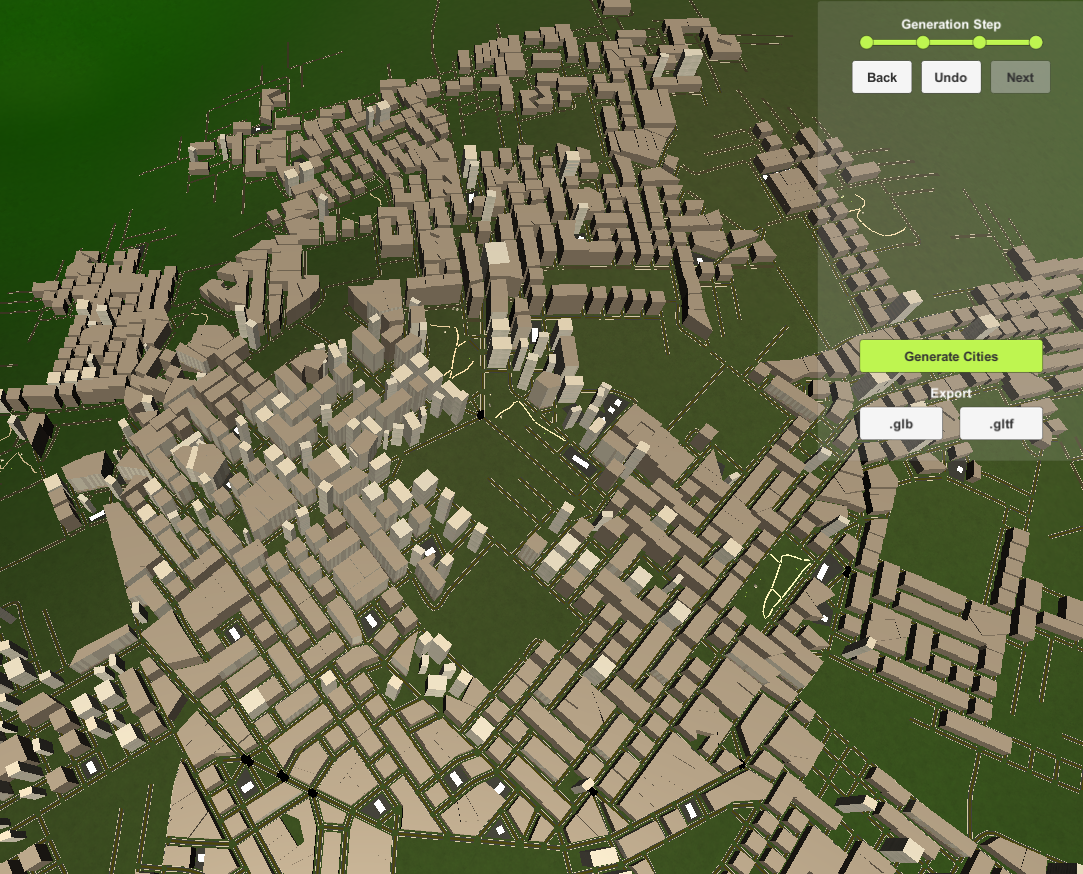
\includegraphics[width=\textwidth]{figure/results/city_paris.png}
      \caption{Example of a fully generated Paris-style city.}
      \label{fig:results_city_paris}
    \end{minipage}
  \end{minipage}
  \begin{minipage}{.45\textwidth}
    \begin{minipage}{.9\textwidth}
      \centering
      \centering
      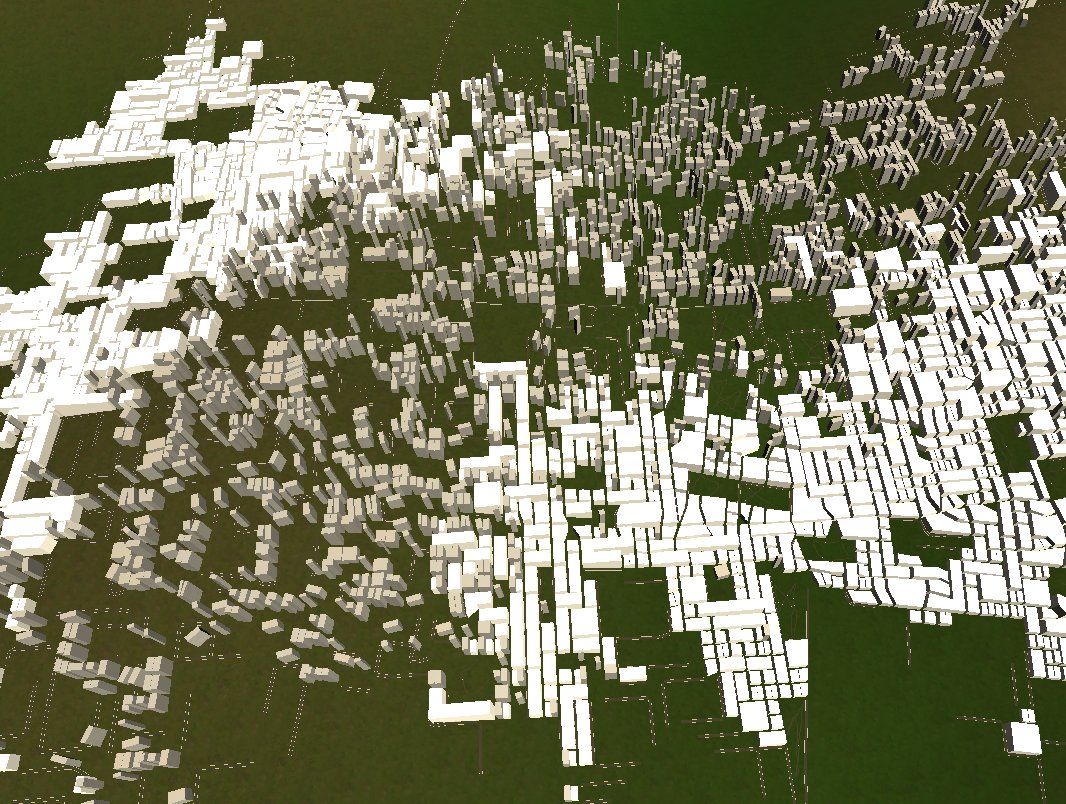
\includegraphics[width=\textwidth]{figure/results/city_manhattan.png}
      \caption{Example of a fully generated Manhattan-style city.}
      \label{fig:results_city_manhattan}
    \end{minipage}
  \end{minipage}
\end{figure}

Both city types uses the population map for different decisions that the Agents makes during the course of their lifetime.
Roads outside the bounds of the city navigates towards higher density areas while roads inside the bounds are shaped to some degree according to the population map.
For example, the streets are not always created when the population is too low.
